%! TEX root = ../main.tex
\documentclass[../main]{subfiles}

% ローカル下書き用
% \documentclass{supernova_pre}
% このクラスの中に大体のパッケージは入ってるので基本何でもかけるはず
% 追加したいパッケージがあればここに記入


\begin{document}
\chapter{インターバル撮影を楽にしたい!!} % タイトル
\rightline{M1 丸山颯斗} % 学年と名前(ハンドルネームでも可)
\section{動機}
普段僕は天体写真を中心に撮影を行っています。天体写真では銀河や星雲などのとても淡い(暗くて観測しづらい)ものを撮影します。月のような明るいものであれば、1枚でもそこそこにきれいな写真になりますが、天体写真では同じ設定で写真を何枚も撮影します。今回の本筋からは逸れてしまうため簡単な説明で済ませると、天体など暗いものを撮ろうとしたときにはノイズを抑えるために写真をたくさん撮影し、それらを編集することが一般的です。そのため自分も天体を撮るときにはきれいな天体写真にするためにたくさんの写真を撮っています。たくさん写真を撮るのは正直とても骨の折れる作業で、1枚の写真を撮るたびにリモートシャッターのボタンを押すことをしています。写真は少なくとも50枚程度は撮りたいのですが、いつも手動でシャッターを切るのが面倒であるため、この作業を楽にしようというのが今回のテーマになります。ちなみに自動でシャッターを切ってくれるデバイスは存在するのですが、僕が使用しているカメラCanon EOS Kiss M2ではカメラ側が対応していないのでこの苦行を強いられています。

\section{目標}
そこで今回目標とするのは既製品で売られているリモートシャッターを使ってインターバル撮影ができるようにすることです。シャッター間隔、シャッター枚数、シャッター時間の3つを自由に設定できることを最低要件として制作を行いました。

\section{制作}
制作の方針としては既製品のリモートシャッター(Canon BR-E1)のシャッターボタンの押し判定をマイコン(Arduino)で制御する方向性で行いました。Canon EOS Kiss M2ではシャッターレリーズ用の端子がなく、Bluetoothリモコンでしかシャッターを切れないこととBluetoothでカメラ本体と接続することの困難さからこのような手法を取りました。また改造するにあたって電子工作の技術が必要となりますが、未経験でもボタンの押し判定を制御するぐらいなら簡単だろうと割と楽観的な考えで取り掛かり始めました。

\subsection{材料}
制作に必要なものは以下です。電子工作のための機材購入等もあり、費用は1万円以上はかかりました。
\begin{itemize}
\item Canon BR-E1
\item Arduino UNO(互換品)
\item ユニバーサル基板
\item LCDディスプレイモジュール
\item スイッチ類(操作用、ディスプレイ用)
\item トランジスタ
\end{itemize}
その他電子工作なのでテスター、抵抗、ハンダゴテ、導線などが必要でした。

\subsection{制御プログラム}
単なるボタンの押し判定をさせるだけでなくインターバル撮影の設定を変更できるようにしたかったため、ボタン操作で変更できる簡単な制御プログラムを作成しました。Arduino IDEというソフトウェアを使ってマイコンに書き込みます。


\subsection{基盤実装}
制御プログラムができて、ブレッドボードでのテストも成功し、最後に完成品として実装を行いました。回路図を\textbf{図}\ref{kairozu}に示しました。電気回路は全然専門でなく、電子工作も初めてだったので有識者の方々は大目に見てください。スイッチやトランジスタ周りは正しい書き方を知らないので適当に解釈してください。\\
 回路図の右上がシャッターボタンを扱う部分です。Arudionoの2番ピンでトランジスタを操作することでBR-E1のスイッチの回路を短絡させて、シャッターボタンを押したときと同じ動作を実現しています。下部はステータスや設定を表示するLCDディスプレイです。右にはその設定を変更するためのスイッチ類で、タクトスイッチを用いました。その他にも回路図には書いていませんが、電源なしでシャッターボタンを押すための別スイッチやディスプレイのバックライトを消すためのロッカースイッチも実装しました。撮影中は周りの迷惑にならないようにディスプレイを暗くできます。

\begin{figure}
    \centering
    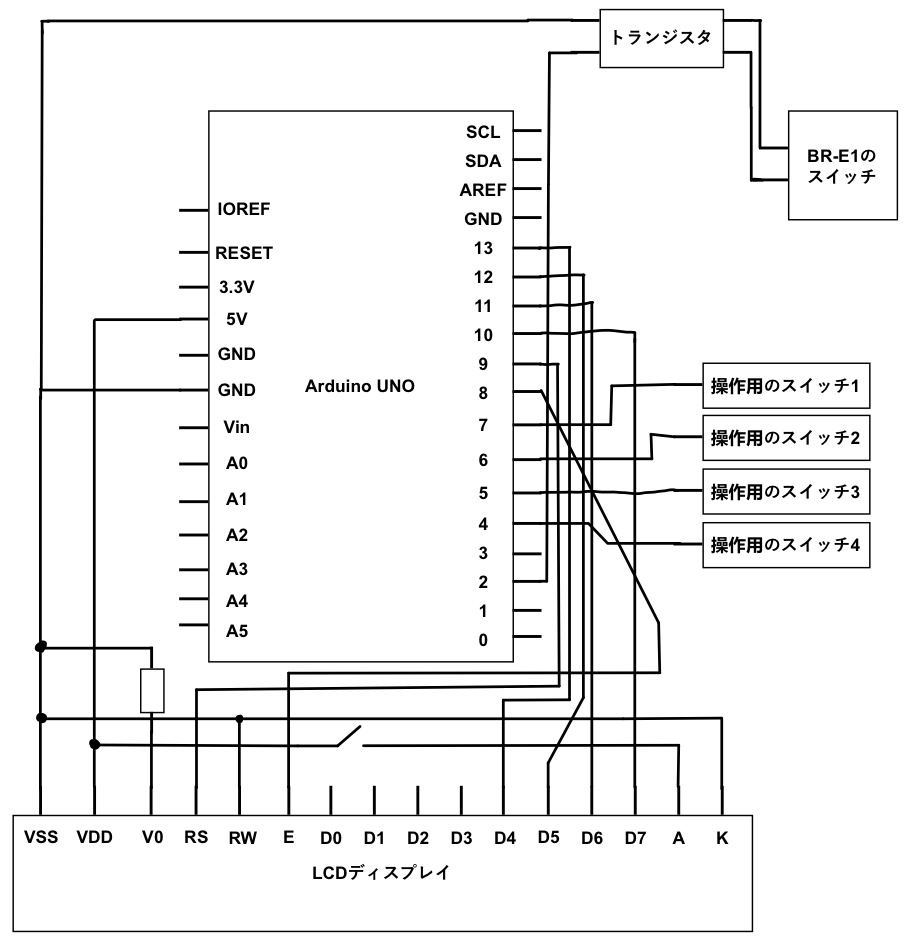
\includegraphics[width=0.5\linewidth]{sections/Maruyama/figure/kairozu.png}
    \caption{実装した回路図モドキ}
    \label{kairozu}
\end{figure}

\subsection{完成品}
\textbf{図}\ref{kansei}が完成の写真です。なかなか回路が複雑だったので、一番下にマイコン、真ん中に配線とBR-E1、一番上にスイッチ類とディスプレイという構成になりました。厚さはそこそこありますが、ある程度いい形にできたのかなと思います。

\begin{figure}
    \centering
    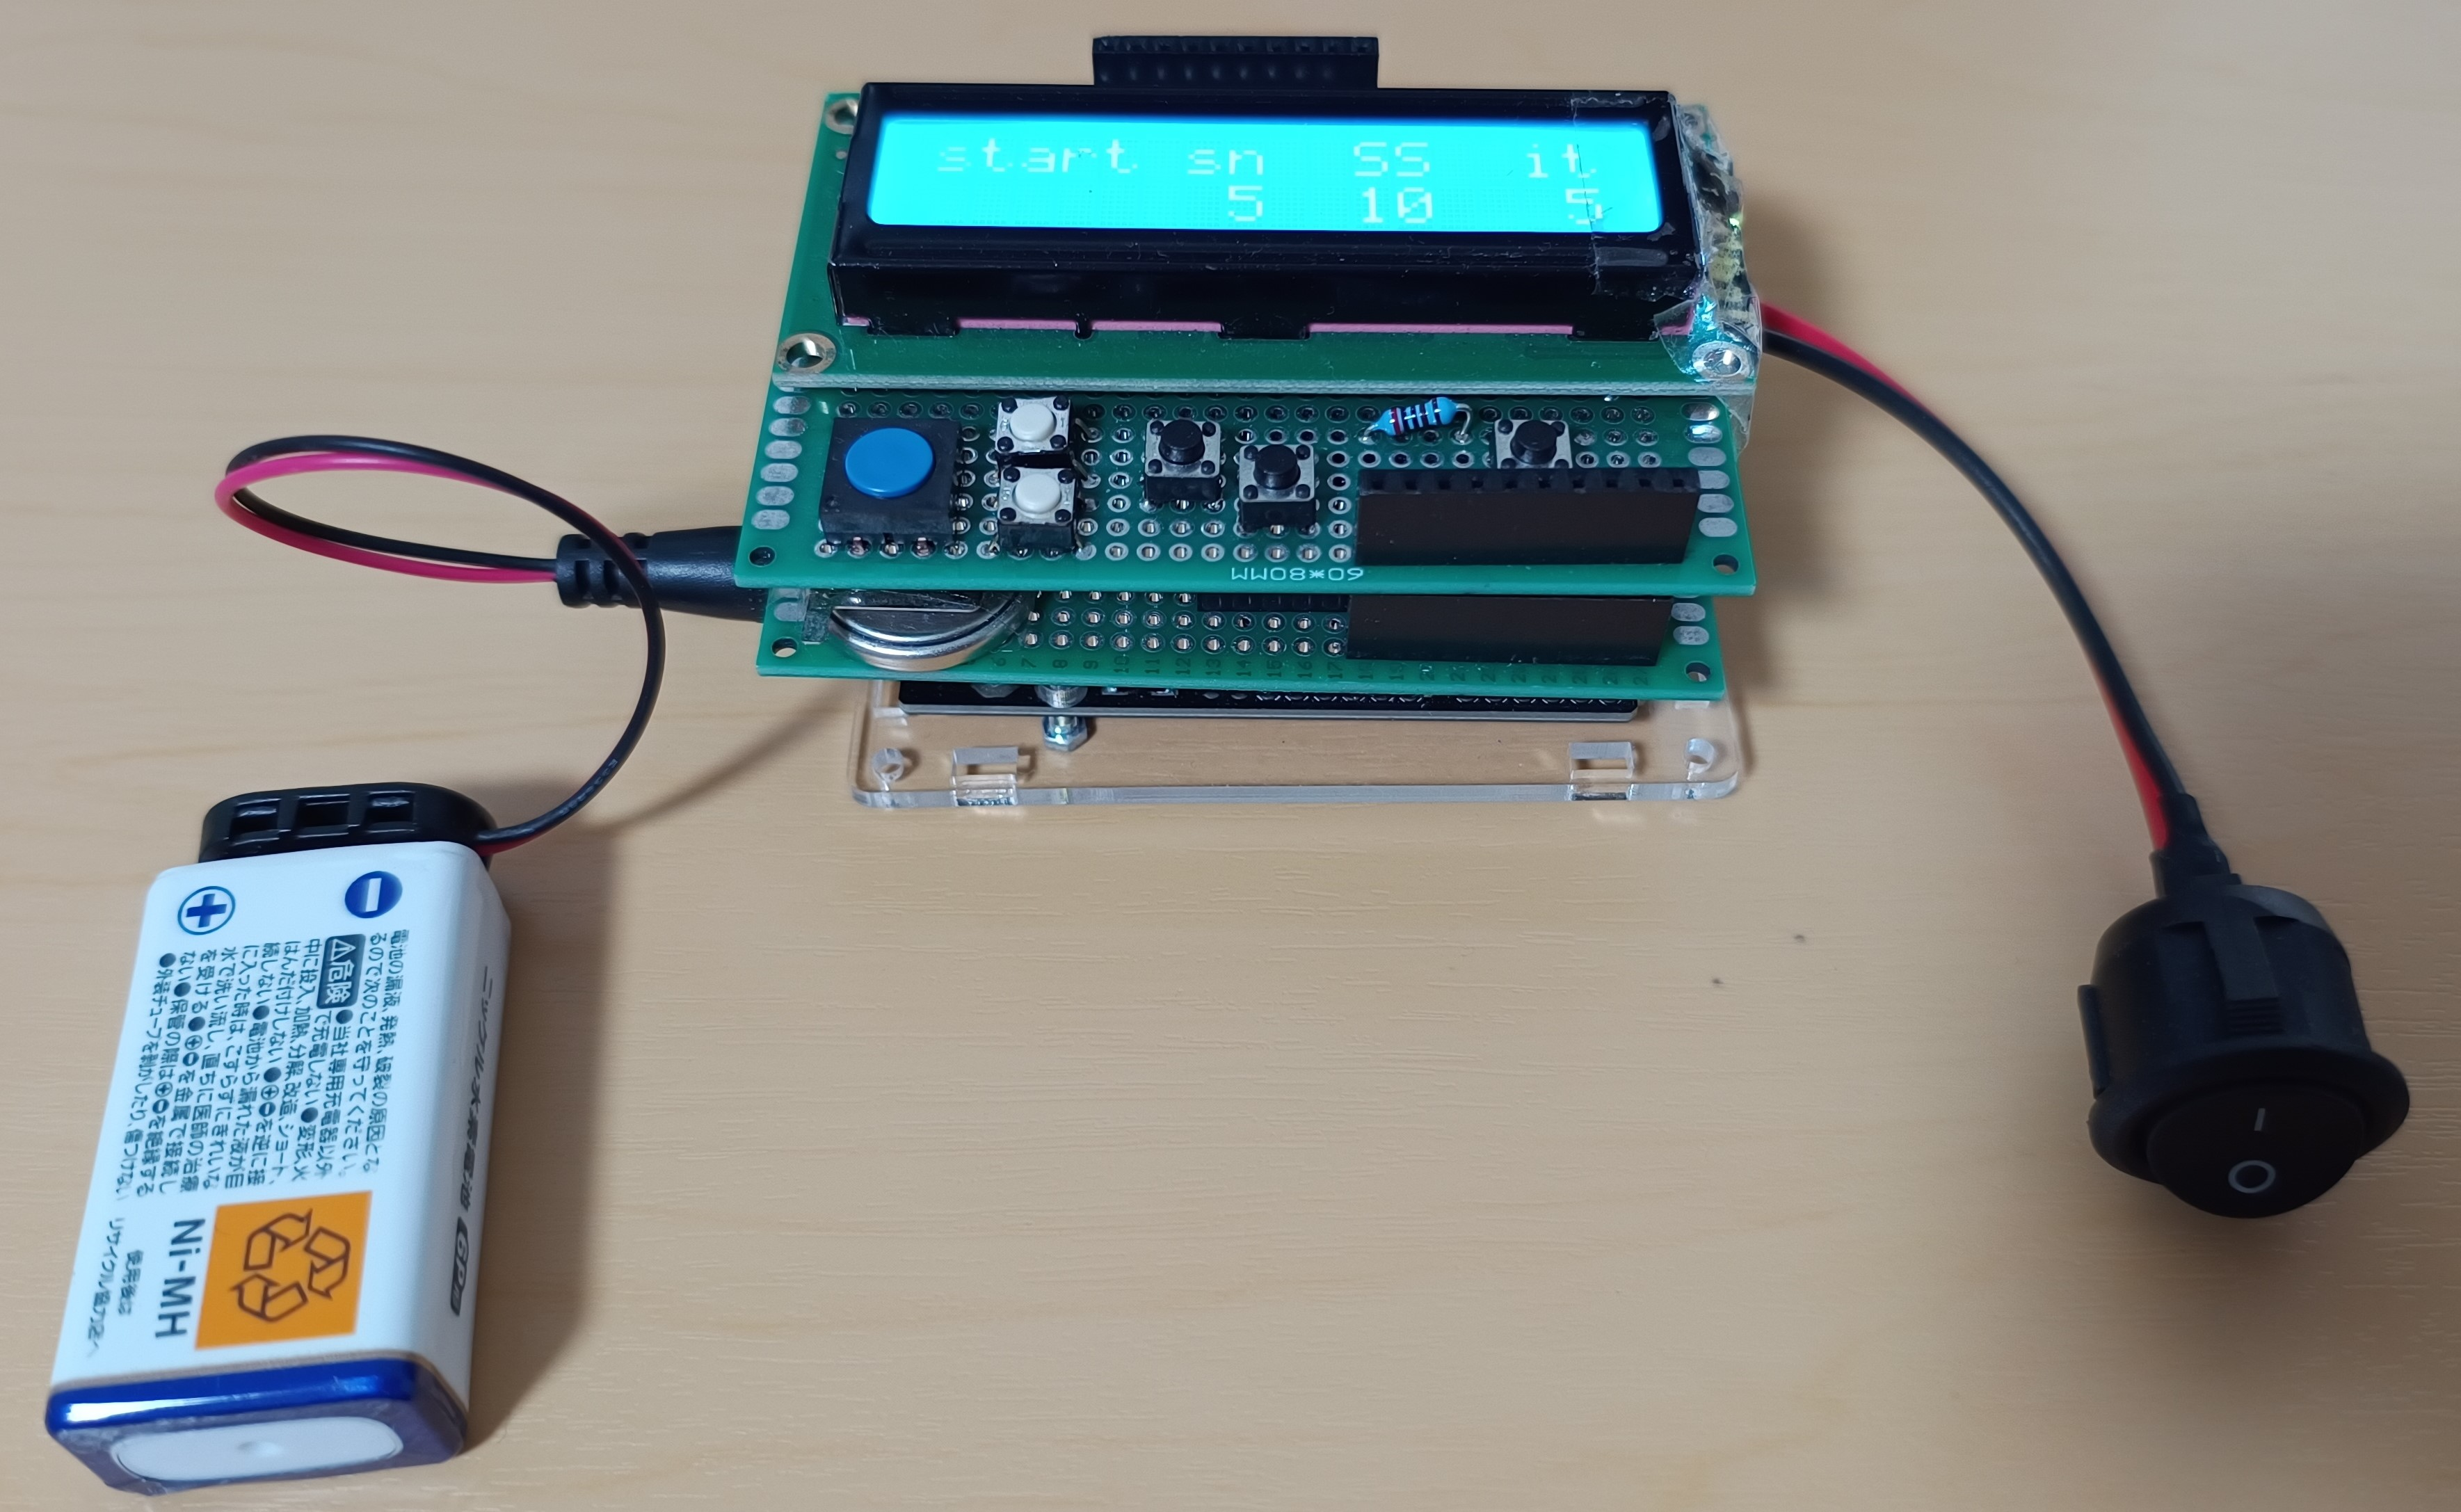
\includegraphics[width=0.5\linewidth]{sections/Maruyama/figure/zentai.jpg}
    \caption{完成品の全体像}
    \label{kansei}
\end{figure}
\textbf{図}\ref{jikkou}が実際に撮影中のディスプレイの表示です。Shootingとかいう文字で撮影中を表し、シャッタースピードにはSS(Shutter Speed)、インターバル時間にはit(interval time)とかいう英語を充ててます。左下のtookとかいうのは撮った枚数のつもりです。

\begin{figure}
    \centering
    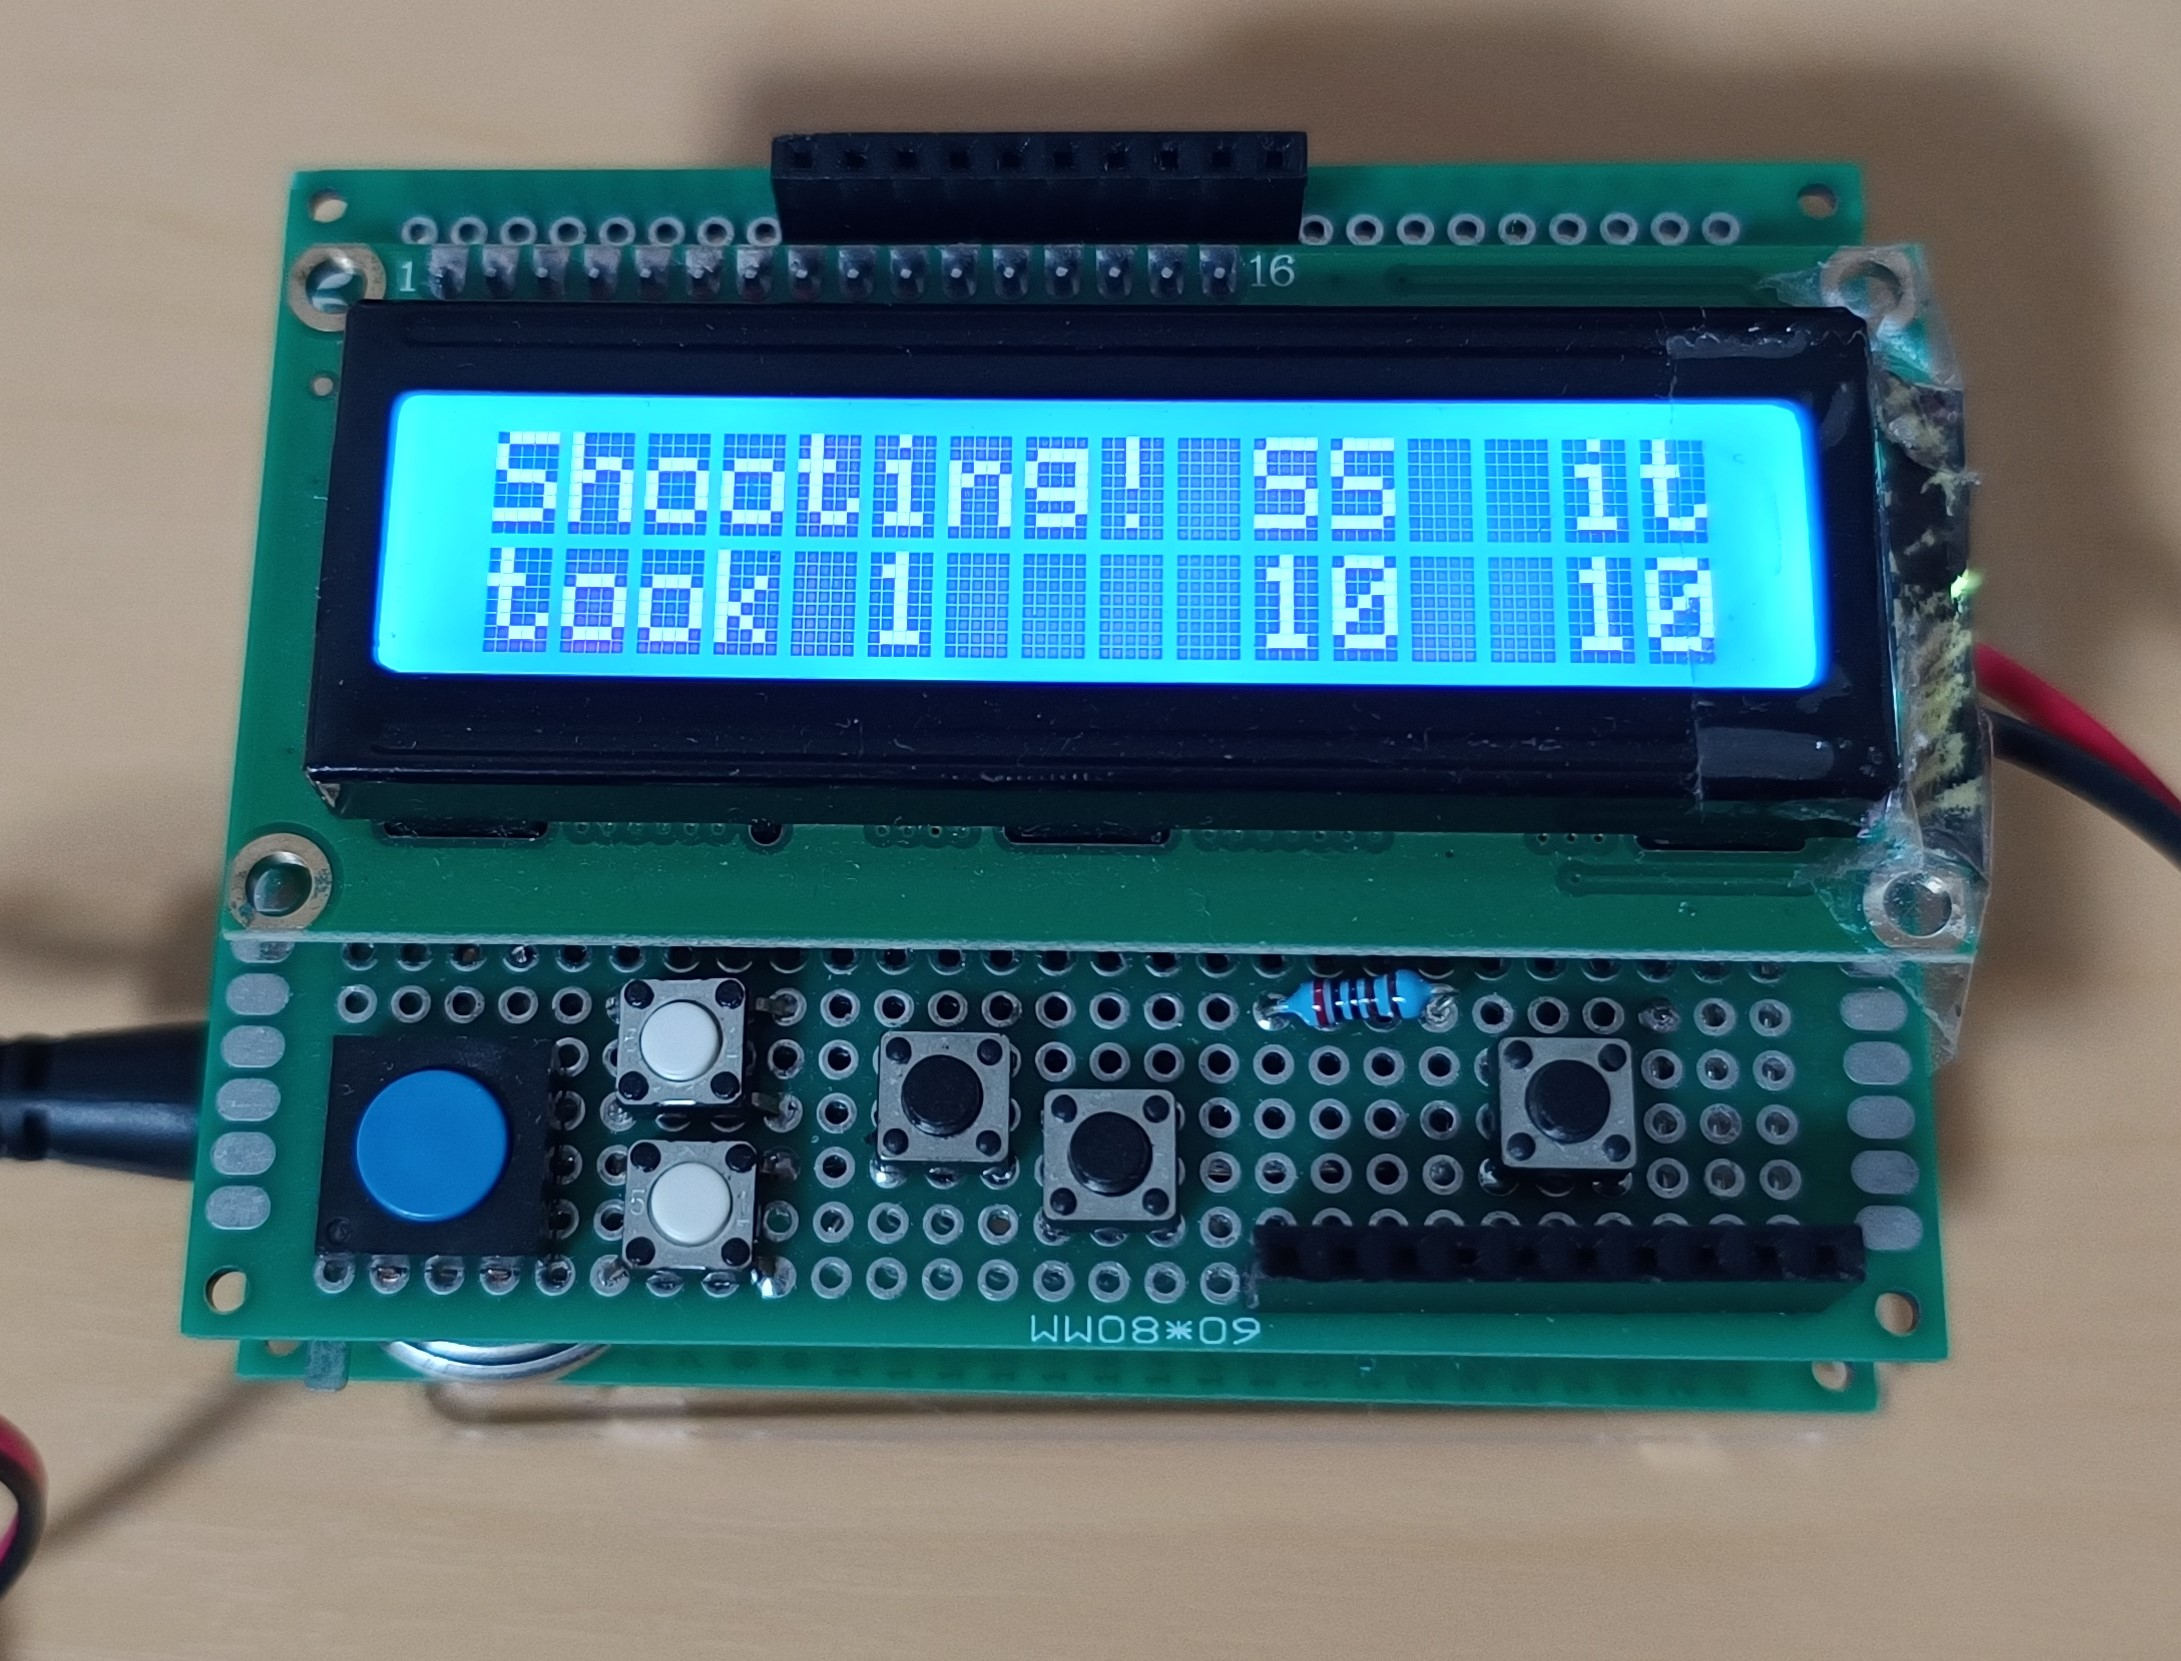
\includegraphics[width=0.5\linewidth]{sections/Maruyama/figure/jikkou.jpg}
    \caption{撮影中のディスプレイ}
    \label{jikkou}
\end{figure}

\section{使用}
完成したものを実際に撮影に使用してみました。使い心地の感想としては「すばらしい!!求めてたものだ!!」です。大満足です。革命です。設定すれば放置するだけでずっと勝手に撮影がされる、これ以上素晴らしいことがあるだろうか、いやない。ただ全てが満足というわけではなくて、気温が低い環境だと上手く動作しないことが複数回ありました。恐らくバッテリーの電圧が足りないか、抵抗値の低下かそのあたりが原因だと思われます。このままでは温かい季節のときしか使えないので、また気が向いたときに修正をしたいです。寒いときでも正常に使えれば双子座流星群のときにも大活躍しそうです。撮影したM101を載せておきます。
\begin{figure}[H]
    \centering
    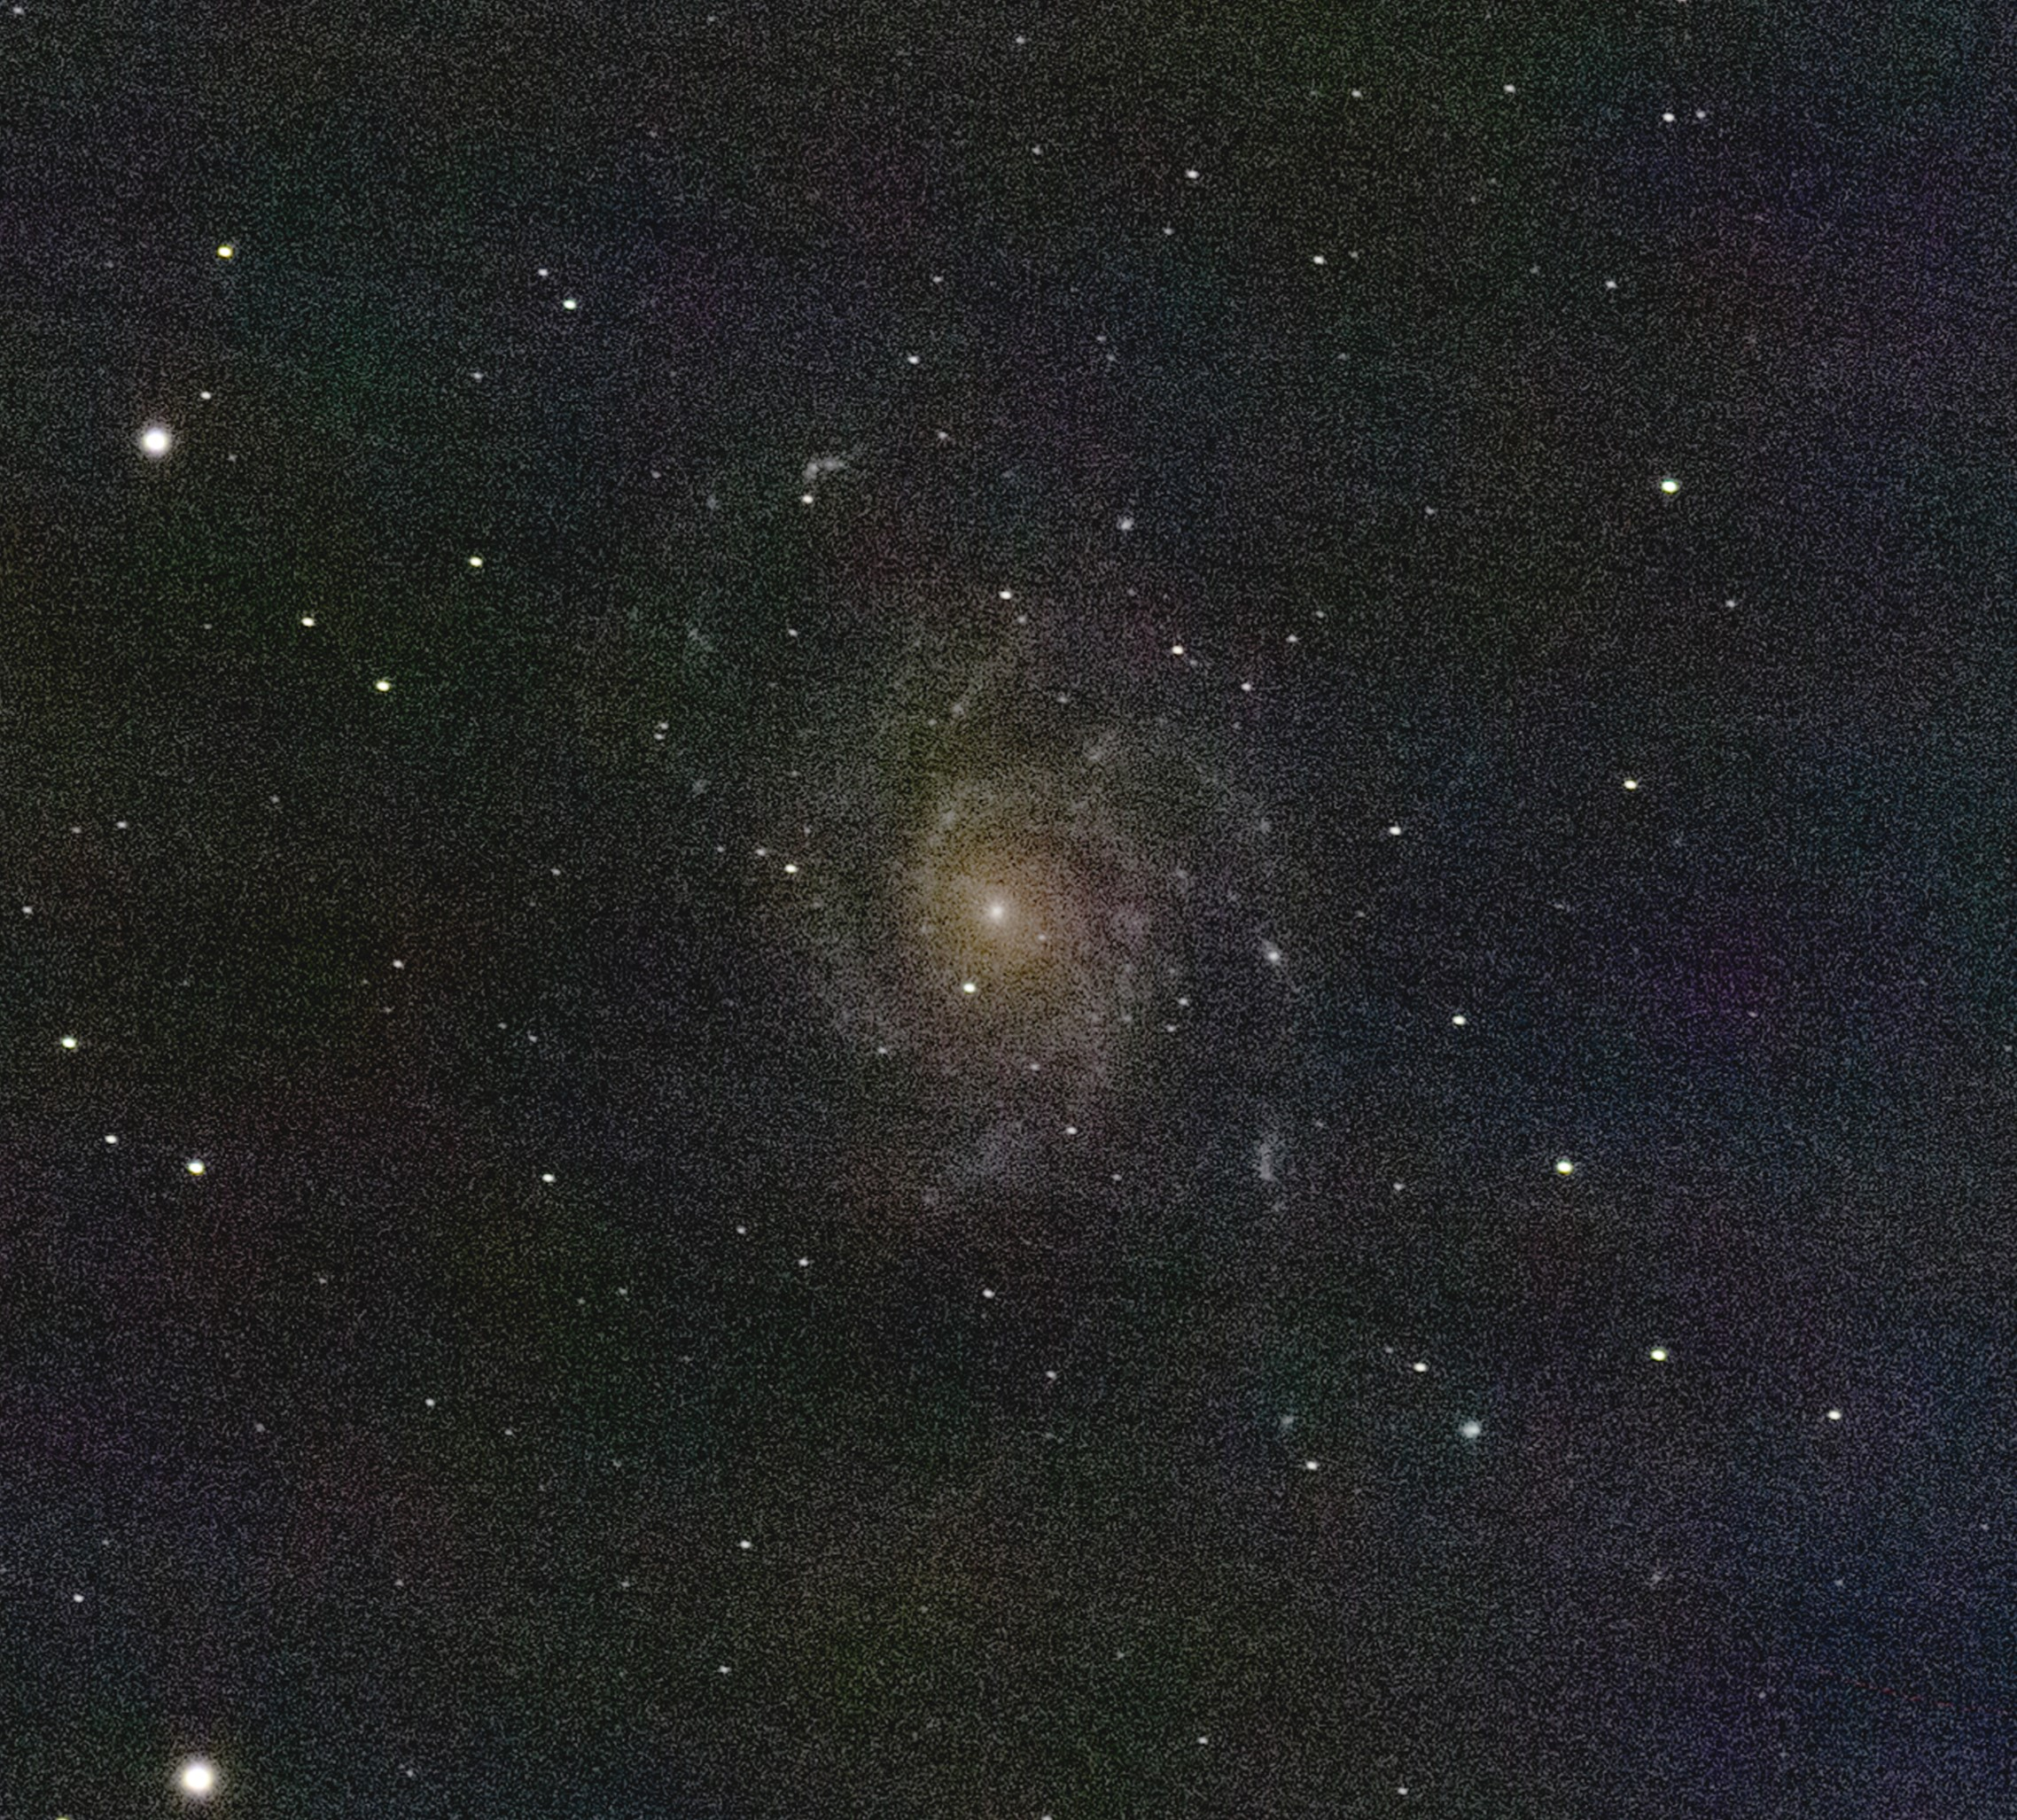
\includegraphics[width=0.5\linewidth]{sections/Maruyama/figure/M101_0529_4.jpg}
    \caption{東3号館屋上にて撮影したM101回転花火銀河}
\end{figure}


\section{まとめ}
天体撮影のインターバル撮影を簡単にしたいという動機から、既製品のリモートシャッターをマイコンで制御することにより、撮影の手間を大幅に軽減することができました。電子工作は初めてで本文では割愛した苦労もありましたが、無事に完成することができ良かったです。ちなみに作成したのはちょうど1年前ぐらいですが、撮影の機会がなくほとんど使っていません。

% \section*{付録}
% \begin{lstlisting}
% const int Interval_time_max=995;//最大インターバル時間
% const int Shot_num_max=995;//最大撮影枚数
% const int Shutter_speed_max=300;//最大シャッタースピード
% long Interval_time=5;//IT
% int Shot_num=5;//SN
% long Shutter_speed=10;//SS


% const int cm=6;//モード変更用端子番号
% const int up=4;//増加用端子番号
% const int down=7;//減少用端子番号
% const int st=5;//スタート用端子番号
% const int shutter_pin=2;

% const int delay_time=400;


% //0が初期(撮影スタート可)、、2がシャッター枚数、3がシャッタースピード
% const int mode_start=0;
% const int mode_SS=1;
% const int mode_sn=2;
% const int mode_it=3;

% int Mode=mode_start;

% #include<LiquidCrystal.h>

% LiquidCrystal lcd(9,8,13,12,11,10);

% void delay_(unsigned long i){//自前delay関数
%   unsigned long t=millis();
%   while((millis() - t) < i){
%     ;
%   }
% }


% void printnow(){//今の設定の状態を表示(モードによって変化)
%   int i=0;
%   lcd.clear();
%   if(Mode==mode_SS || Mode==mode_start){
%     lcd.setCursor(10,0);
%     lcd.print("SS");
%   }
%   if(Mode==mode_sn || Mode==mode_start){
%     lcd.setCursor(6,0);
%     lcd.print("sn");
%   }
%   if(Mode==mode_it || Mode==mode_start){
%     lcd.setCursor(14,0);
%     lcd.print("it");
%   }
%   if(Mode==0){
%     lcd.setCursor(0,0);
%     lcd.print("start");
%   }
%   if(Shutter_speed < 100){
%     i=1;
%   }
%   lcd.setCursor(9+i,1);
%   lcd.print(Shutter_speed);
%   i=0;
%   if(Shot_num < 10){
%     i=2;
%   }else if(Shot_num < 100){
%     i=1;
%   }
%   lcd.setCursor(5+i,1);
%   lcd.print(Shot_num);
%   i=0;
%   if(Interval_time < 10){
%     i=2;
%   }else if(Interval_time < 100){
%     i=1;
%   }
%   lcd.setCursor(13+i,2);
%   lcd.print(Interval_time);
% }


% void up_count(){//ボタンが押されたときの数字を大きくする
%   if(Mode==1){
%     Shutter_speed = Shutter_speed + 10;
%     if(Shutter_speed > Shutter_speed_max){
%       Shutter_speed = 10;
%     }
%   }else if(Mode==2){
%     Shot_num = Shot_num + 5;
%     if(Shot_num > Shot_num_max){
%       Shot_num = 5;
%     }
%   }else if(Mode==3){
%     Interval_time = Interval_time + 5;
%     if(Interval_time > Interval_time_max){
%       Interval_time = 5;
%     }
%   }
%   printnow();
% }

% void down_count(){//ボタンが押されたときの数字を小さくする
%   if(Mode==mode_SS){
%     Shutter_speed = Shutter_speed - 10;
%     if(Shutter_speed < 1){
%       Shutter_speed = Shutter_speed_max;
%     }
%   }else if(Mode==mode_sn){
%     Shot_num = Shot_num - 5;
%     if(Shot_num < 1){
%       Shot_num = Shot_num_max;
%     }
%   }else if(Mode==mode_it){
%     Interval_time = Interval_time - 5;
%     if(Interval_time < 1){
%       Interval_time = Interval_time_max;
%     }
%   }
%   printnow();
% }


% void print_taked(int taked_num){//撮影中用の表示関数
%   int i=0;
%   lcd.setCursor(0,1);
%   lcd.print("took");
%   lcd.setCursor(5,1);
%   lcd.print(taked_num);
%   if(Shutter_speed < 100){
%     i=1;
%   }
%   lcd.setCursor(9+i,1);
%   lcd.print(Shutter_speed);
%   i=0;
%   if(Interval_time < 10){
%     i=2;
%   }else if(Interval_time < 100){
%     i=1;
%   }
%   lcd.setCursor(13+i,2);
%   lcd.print(Interval_time);
% }

% void print_shooting(int i){//撮影中の1行目の表示
%   lcd.clear();
%   lcd.setCursor(0,0);
%   lcd.print("Shooting! SS  it");
%   print_taked(i);
% }

% void shutter(){//シャッターボタンを通電させる
%   digitalWrite(shutter_pin,HIGH);
%   delay(100);
%   digitalWrite(shutter_pin,LOW);
%   delay_(Shutter_speed*1000);
%   if(Shutter_speed > 30){//BULB撮影で閉じる用
%     digitalWrite(shutter_pin,HIGH);
%     delay(100);
%     digitalWrite(shutter_pin,LOW);
%   }
% }

% void shooting(){//撮影中
%   int i=0;
%   print_shooting(i);
%   i++;
%   while(i < Shot_num+1){
%     shutter();
%     print_shooting(i);
%     i++;
%     if(i==Shot_num+1){
%       break;
%     }
%     delay_(Interval_time*1000);
%   }
%   lcd.clear();
%   lcd.setCursor(0,0);
%   lcd.print("Finished! SS  it");
%   print_taked(i-1);
%   while(1){
%   }

% }


% void ready_shutter(){//撮影スタートモード
%   printnow();
%   while(1){
%     if(digitalRead(cm)==0){
%     delay(delay_time);
%     Mode=mode_sn;
%     break;
%     }
%     if(digitalRead(st)==0){
%       delay(delay_time);
%       shooting();
%     }
%   }
% }

% void change_SS(){//シャッタースピード変更モード
%   printnow();
%   while(1){
%     if(digitalRead(cm)==0){
%       delay(delay_time);
%       Mode=mode_it;
%       break;
%     }
%     if(digitalRead(up)==0){
%       delay(delay_time);
%       up_count();
%     }
%     if(digitalRead(down)==0){
%       delay(delay_time);
%       down_count();
%     }
%   }
% }

% void change_sn(){//撮影枚数変更モード
%   printnow();
%   while(1){
%     if(digitalRead(cm)==0){
%       delay(delay_time);
%       Mode=mode_SS;
%       break;
%     }
%     if(digitalRead(up)==0){
%       delay(delay_time);
%       up_count();
%     }
%     if(digitalRead(down)==0){
%       delay(delay_time);
%       down_count();
%     }
%   }
% }

% void change_it(){//インターバル時間変更モード
%   printnow();
%   while(1){
%     if(digitalRead(cm)==0){
%       delay(delay_time);
%       Mode=mode_start;
%       break;
%     }
%     if(digitalRead(up)==0){
%       delay(delay_time);
%       up_count();
%     }
%     if(digitalRead(down)==0){
%       delay(delay_time);
%       down_count();
%     }
%   }
% }

% void setup() {
%   pinMode(cm,INPUT_PULLUP);//モード変更用
%   pinMode(up,INPUT_PULLUP);//カウント増やす用
%   pinMode(down,INPUT_PULLUP);//カウント減らす用
%   pinMode(st,INPUT_PULLUP);//スタートストップ用
%   pinMode(shutter_pin,OUTPUT);//シャッター用
%   lcd.begin(16,2);
% }

% void loop() {
%   if(Mode==mode_start){
%     ready_shutter();
%   }
%   if(Mode==mode_SS){
%     change_SS();
%   }
%   if(Mode==mode_sn){
%     change_sn();
%   }
%   if(Mode==mode_it){
%     change_it();
%   }
%   // put your main code here, to run repeatedly:

% }

% \end{lstlisting}
\end{document}